% resume.tex - My personal resume

%check to see if we defined the resume document class from the command line
%if so, do nothing. If not, define it to be in draft mode.
\makeatletter
\@ifclassloaded{resume}
  {}
  {\documentclass[draft]{resume}}
\makeatother

\usepackage[headheight=24pt, headsep=10pt, letterpaper, portrait, top=1in, bottom=0.75in, left=0.5in, right=0.5in]{geometry}
\usepackage{graphicx}
\usepackage{hyperref}

\graphicspath{{./img/}}
\pagestyle{fancy}
\fancyfoot[R]{Built with \LaTeX}
\addtolength{\parskip}{-0.5mm}

\begin{document}
  \name{Aaron Pittenger \href{https://github.com/pittenga/resume}{
\includegraphics[keepaspectratio, height=2ex]{github.png}} \href{https://www.linkedin.com/in/pittenga}{
\includegraphics[keepaspectratio, height=2ex]{linkedin.png}}}
  \address{2665 Burgen Ave NE}{Grand Rapids, MI 49525}
  \contact{aaron.pittenger@ge.com}{+1.517.937.5543}

  \pagenumbering{gobble}

  \resumesection{Education}
  \education{2010 - 2013}{Marquette University - Milwaukee, WI}{Masters of Science in Computing - GPA: 4.0}
  \education{2010 - 2013}{GE Edison Engineering Development Program - Grand Rapids, MI}{Accredited, company taught courses in advanced software engineering topics}
  \education{2005 - 2010}{Grand Valley State University - Allendale, MI}{Bachelor of Science in Computer Engineering - GPA: 3.235}

  %TODO: Add links to companies and stuff I've worked on.
  \resumesection{Experience}

  %TODO: Make sure everything that should be in here is in here.
  \begin{experience}{Aug 2010 - Present}{GE Aviation Systems - Grand Rapids, MI}{Senior Software Engineer, Software Engineer, Edison Engineering Development Program}{ge.png}
    \task{Led SW development on multiple projects including planning, forecasting, earned value management and milestone tracking}
    \task{Lead developer for multiple features on multiple projects}
    \task{Embedded software developer utilizing VxWorks, Linux and bare metal OS}
    \task{Device driver implementation on multiple platforms}
    \task{Designed and created an automated testing/continuous integration plan for multiple projects}
    \task{Lead continuous improvement initiative for group, saving over \$1MM in 2 years}
  \end{experience}

  \begin{experience}{Jun 2014 - Present}{MichiganLabs - Grand Rapids, MI}{Application Developer}{ml.png}
    \task{Full lifecycle enterprise projects (iOS and Android) from customer requirements through final app publication}
    \task{Released applications:}
    \item[] %Blank item here makes everything format a little nicer.
    \begin{tabular}{ c c c c }
        GiveAWow & 360 Recognition & Light of Life & WCSG 91.3
    \end{tabular}
  \end{experience}

  \begin{experience}{Aug 2011 - Dec 2011}{Grand Valley State University - Grand Rapids, MI}{School of Engineering - Adjunct Faculty}{gvsu.png}
    \task{Lab instructor for Introduction to Digital Systems (EGR 226)}
    \task{Assisted students during lab and graded lab assignments weekly}
  \end{experience}

  \begin{experience}{Jan 2009 - Aug 2010}{GE Aviation Systems - Grand Rapids, MI}{Systems Engineering - Intern}{ge.png}
    \task{Worked on military aircraft Flight Management System (FMS) requirements management}
    \task{Facilitated weekly meetings with customer (Lockheed Martin) to review requirements and discuss potential problems}
    \task{Created a Multifunction Control Display Unit (MCDU) emulator that generates requirements automatically to speed up requirements process and increase customer satisfaction}
  \end{experience}

  \begin{experience}{May 2008 - Aug 2008}{GE Healthcare - Waukesha, WI}{Service Methods Design Engineer - Intern}{ge.png}
    \task{Programmed an illustrated replaceable parts list tool}
    \task{This tool saves GEHC ~ \$5.5MM in time wasted by field service personnel using the paper parts lists to look up replacement parts on machines}
    \task{Enhanced the look and feel of a System Error Log Viewer}
    \task{Prepared all necessary paperwork for the release of both tools mentioned above}
    \task{Hands-on training with writing validation and verification procedures on PET/CT Scanners}
  \end{experience}

  %TODO: Add additional interests and hone in on skills.
  \resumesection{Skills}
  \begin{skills}
    
\includegraphics[keepaspectratio, height=1cm]{c.png}
    
\includegraphics[keepaspectratio, height=1cm]{c++.png}
    
\includegraphics[keepaspectratio, height=1cm]{ada.png}
    
\includegraphics[keepaspectratio, height=1cm]{java.png}
    
\includegraphics[keepaspectratio, height=1cm]{objc.png}
    
\includegraphics[keepaspectratio, height=1cm]{python.png}
    
\includegraphics[keepaspectratio, height=1cm]{shell.png}
    
\includegraphics[keepaspectratio, height=1cm]{html.png}
    
\includegraphics[keepaspectratio, height=1cm]{latex.png}
    
\includegraphics[keepaspectratio, height=1cm]{lua.png}
    
\includegraphics[keepaspectratio, height=1cm]{linux.png}
    
\includegraphics[keepaspectratio, height=1cm]{apple.png}
    
\includegraphics[keepaspectratio, height=1cm]{windows.png}
    
\includegraphics[keepaspectratio, height=1cm]{ubuntu.png}
    
\includegraphics[keepaspectratio, height=1cm]{android_studio.png}
    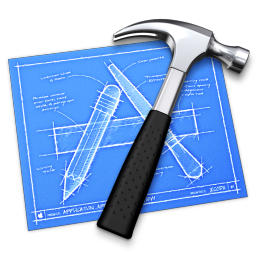
\includegraphics[keepaspectratio, height=1cm]{xcode.png}
    
\includegraphics[keepaspectratio, height=1cm]{atlassian.png}
    
\includegraphics[keepaspectratio, height=1cm]{eclipse.png}
    
\includegraphics[keepaspectratio, height=1cm]{git.png}
    
\includegraphics[keepaspectratio, height=1cm]{subversion.png}
    
\includegraphics[keepaspectratio, height=1cm]{gnu.png}
    
\includegraphics[keepaspectratio, height=1cm]{jenkins.png}
    
\includegraphics[keepaspectratio, height=1cm]{office.png}
    
\includegraphics[keepaspectratio, height=1cm]{virtualbox.png}
    
\includegraphics[keepaspectratio, height=1cm]{vmware.jpg} \\
  \end{skills}

  \resumesection{Training}
  GE Foundations of Leadership, GE Customer Technical Presentation Skills, GE Leadership Development Course

  \resumesection{Interests}
  Project Management, Embedded Products, SW Development Process, Dev Ops, Continuous Integration/Delivery, Process Improvement

\end{document}
